\documentclass{beamer}
\usepackage{../common_slides}

\title{Text Classification\\ + \\ Machine Learning Review 3 }
\date{}
\author{CS 287}
\begin{document}

\begin{frame}
  \titlepage
\end{frame}

\begin{frame}{Review: Gradients for Softmax Regression}

  For multiclass logistic regression:
  
  \[ \frac{\partial L(\boldy, \hat{\boldy})}{\partial z_i} = \sum_{j} \frac{\partial \hat{y}_j }{\partial z_i}  \frac{\indicator(j = c)} {\hat{y}_j} =     \begin{cases}
      -(1 - \hat{y}_i) & i = c\\
      \hat{y}_i & ow. \\
    \end{cases} \] 

  Therefore for parameters $\theta$, 

  \[\frac{\partial L}{\partial b_{i}} = 
    \frac{\partial L}{\partial z_{i}} \ \ \ \ \frac{\partial L}{\partial W_{f, i}} = 
     x_f \frac{\partial L}{\partial z_{i}}\]

   \pause
   Intuition:
   \begin{itemize}
   \item Nothing happens on correct classification.
   \item Weight of true features increases based on prob not given.
   \item Weight of false features decreases based on prob given.
   \end{itemize}
\end{frame}


\begin{frame}{Gradient-Based Optimization: SGD}
  \begin{figure}
    \begin{algorithmic}
      \Procedure{SGD}{}
      \While{training criterion is not met}
      \State{Sample a training example $\boldx_i, \boldy_i$}
      \State{Compute the loss $L(\hat{\boldy}_i, \boldy_i;\theta)$}
      \State{Compute gradients $\hat{\boldg}$ of $L(\hat{\boldy}_i, \boldy_i;\theta)$ with respect to $\theta$}
      \State{$\theta \gets \theta - \eta \hat{\boldg}$}
      \EndWhile{}
      \State{\Return{$\theta$}}
      \EndProcedure{}
    \end{algorithmic}
  \end{figure}
\end{frame}


\begin{frame}{Quiz: Softmax Regression}
  Given bag-of-word features \[\mcF = \{\mathrm{\texttt{The, movie, was, terrible, rocked, A}} \}\] and two training data points:
    
  \begin{center}
    Class 1: \texttt{The movie was terrible}
  
    Class 2: \texttt{The movie rocked}
  \end{center}
  \\

  \air 

  Assume that we start with parameters $\boldW = 0$ and $\boldb = 0$,
  and we train with learning rate $\eta = 1$ and $\lambda = 0$. What is
  the loss and the parameters after one pass through the data in order?
\end{frame}

\begin{frame}{Answer: Softmax Regression (1) }
  First iteration,
  \[\hat{\boldy}_1 = \begin{bmatrix} 0.5 0.5 \end{bmatrix}\]

  \[ L(\boldy_1, \hat{\boldy}_1) = - \log 0.5 \]

  \[ \boldW =
  \begin{bmatrix}
    0.5 & 0.5 & 0.5 & 0.5 & 0 & 0 \\
    -0.5 & -0.5 & -0.5 & -0.5 && 0 & 0 \\
  \end{bmatrix}
  \]

  
  \[ \boldb =
  \begin{bmatrix}
    0.5 & -0.5 \\
  \end{bmatrix} \]
\end{frame}


\begin{frame}{Answer: Softmax Regression (2) }
  Second iteration,

  \[\hat{\boldy}_1 = \softmax([1.5\ -1.5] ) \approx \begin{bmatrix} 0.95 \  0.05  \end{bmatrix}\]

  \[ L(\boldy_2, \hat{\boldy}_2) = - \log 0.05 \]

  \[ \boldW \approx
  \begin{bmatrix}
    -0.45 & -0.45 & 0.5 & 0.5 & -0.95 & 0 \\
     0.45 & 0.45 & -0.5 & -0.5 & 0.95 & 0 \\
  \end{bmatrix}
  \]

  \[ \boldb =
  \begin{bmatrix}
    0.5 & -0.5 \\
  \end{bmatrix} \]
\end{frame}


\begin{frame}{Today's Class}
  So far
  \begin{itemize}
  \item Naive Bayes (Multinomial)
  \item Multiclass Logistic Regression (SGD)
  \end{itemize}

  Today

  \begin{itemize}
  \item Multiclass Hinge-loss
  \item More about optimization
  \end{itemize}
\end{frame}


\section{Multiclass Hinge-Loss}



\begin{frame}{Other Loss Functions}
  
  What if we just try to directly find $\boldW$ and $\boldb$? 
     \[\hat{\boldy} = \boldx \boldW + \boldb\]   
     
     \begin{itemize}
     \item $f(x) = x$ 
     \item No longer a probabilistic interpretation.
     \item Just try to find parameters that fit training data.
     \end{itemize}

\end{frame}

\begin{frame}{Ideal Loss}
  
  
  \[{\mathcal{L}(\theta)} = \sum_{i=1}^n L_{0/1}(\hat{\boldy}, \boldy) \] 

  \[ L(\hat{\boldy}, \boldy) =  \indicator(\argmax_{c'} \hat{y}_{c'} = c) \}  \]
\end{frame}


\begin{frame}{Hinge or ReLU Function}
  \begin{itemize}
  \item \[\relu(z) = \max\{0, z\}  \]
  \end{itemize}

\end{frame}

\begin{frame}{Hinge Loss}

  \[{\mathcal{L}(\theta)} = \sum_{i=1}^n L_{hinge}(\hat{\boldy}, \boldy) \] 


  \[ L(\hat{\boldy}, \boldy) =  \max\{0, 1 - (\hat{y}_{c} + \hat{y}_{c'}) \}  \]

  Where 
  \begin{itemize}
  \item   Let $c$ be defined as true class $y_{i, c} = 1$  
  \item   Let $c'$ be defined as the highest scoring non-true class 
    \[c' = \argmax_{i \in \mcC \setminus\{c\}} \hat{y}_i \] 
  \end{itemize}
\end{frame}

% \begin{frame}{Hinge Loss}
%   For a given example $\boldy_i$,

%   \begin{itemize}
%   \item   Where $c$ is gold class $y_{i, c} = 1$  
%   \item    $\bar{c}$ is the highest scoring non-gold class 
%     \[\bar{c} = \argmax_{c \in \mcC \setminus\{c\}} \hat{y}_c \] 
%   \end{itemize}


%     \[ \mathcal{L}_{margin}(\theta) = \sum_{i=1}^n \max\{0, 1 - \hat{y}_{i, c} + \hat{y}_{i, \bar{c}}\}  + ||\theta||^2_2 \]
% \end{frame}


\begin{frame}{Hinge Loss}
  \begin{columns}[t]
    \begin{column}[t]{0.5\textwidth}


      \begin{figure}
        \centering
        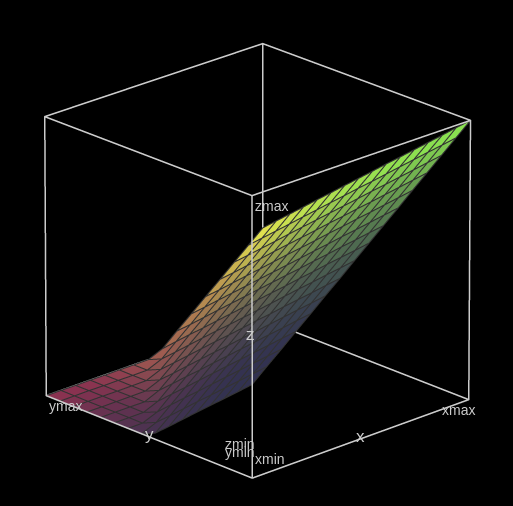
\includegraphics[width=5cm]{hinge}

      \end{figure}
      \[hinge(\hat{\boldy}) = \indicator(\max\{0, 1 - (y - x)) \]
    \end{column}

    \begin{column}[t]{0.5\textwidth}


      \begin{figure}
        \centering
      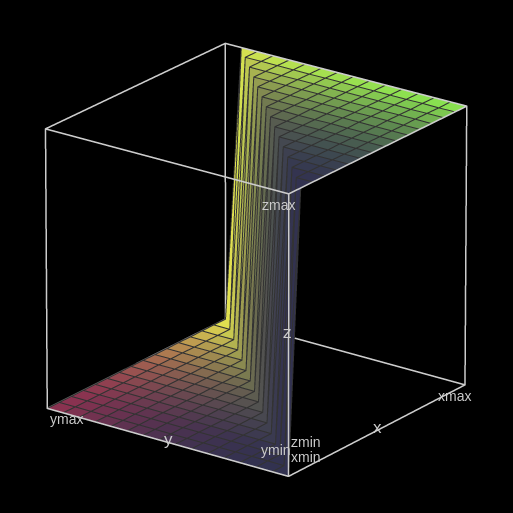
\includegraphics[width=5cm]{argmax}
      \end{figure}
      \[\argmax([x\ y]) = \indicator(x > y) \]      
    \end{column}
  \end{columns}
\end{frame}  




\begin{frame}{Hinge-Loss Properties}
  
\end{frame}


\begin{frame}{Symbolic Gradients}

  \begin{itemize}
  \item   Let $c$ be defined as true class $y_{i, c} = 1$  
  \item   Let $c'$ be defined as the highest scoring non-true class 
    \[c' = \argmax_{i \in \mcC \setminus\{c\}} \hat{y}_i \] 
  \end{itemize}
  
  Much simpler than logistic regression.

  \begin{itemize}
  \item Partials of $L(y, \hat{y})$

  \[ \frac{\partial L(y,k \hat{y})}{\partial \hat{y}_j} = \indicator(j = c) - \indicator(j = c')  \]

   \end{itemize}
\end{frame}


\begin{frame}{Notes: Hinge Loss: Regularization}
  \begin{itemize}
  \item   Many different names,
  \begin{itemize}
  \item Margin Classifier
  \item Multiclass Hinge
  \item Linear SVM
  \end{itemize}

  \item Important to use regularization.  
  \[ \mathcal{L}(\theta) = - \sum_{i=1}^n L(\hat{\boldy}, \boldy) + ||\theta||^2_2\] 

  \item Can be much more efficient to train than LR. (No partition).

  \end{itemize}
\end{frame}


\begin{frame}{Kernels}
  
\end{frame}

\begin{frame}{Results: Longer Reviews}
  \begin{figure}
    \centering
    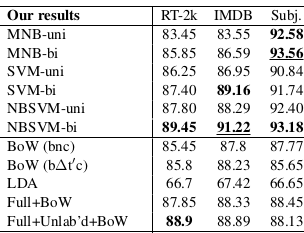
\includegraphics{svm}
    \caption{IMDB (longer movie review), Subj (longer subjectivity)}
  \end{figure}

  \begin{itemize}
  \item NBSVM is hinge-loss interpolated with Naive Bayes.
  \end{itemize}
\end{frame}



\section{Black-Box Optimization}

\begin{frame}{First-Order Methods}
  \begin{itemize}
  \item Minimize function $L(\theta)$
  \item Require computing $L(\theta)$ and gradient $L'(\theta)$.
  \end{itemize}
\end{frame}


\begin{frame}{Gradient Descent}
  \begin{figure}
    \begin{algorithmic}
      \While{training criterion is not met}
      \State{Sample a minibatch of $m$ examples $(\boldx_1, \boldy_1), \ldots, (\boldx_m, \boldy_m) $}
      \State{$\hat{\boldg} \gets 0$}
      \For{$i = 1 \mathrm{\ to\ } m$}
      \State{Compute the loss $L(\hat{\boldy}_i, \boldy_i;\theta)$}
      \State{Compute gradients $\boldg'$ of $L(\hat{\boldy}_i, \boldy_i;\theta)$ with respect to $\theta$}
      \State{$\hat{\boldg} \gets \hat{\boldg} +  \frac{1}{m} \boldg'$}
      \EndFor{}
      \State{$\theta \gets \theta - \eta_k \hat{\boldg}$}
      \EndWhile{}
      \State{\Return{$\theta$}}
    \end{algorithmic}
  \end{figure}  
\end{frame}


\begin{frame}{Stochastic First-Order Methods}
  \begin{itemize}
  \item Minimize function $L(\theta)$
  \item Require computing $L(\theta), $
  \end{itemize}
\end{frame}



\begin{frame}{Stochastic Optimization}
  \begin{itemize}
  \item Select subset of training examples.
  \item Compute gradient of loss
  \item Take step.
  \end{itemize}
\end{frame}


\begin{frame}{Gradient-Based Optimization: Minibatch SGD}
  \begin{figure}
    \begin{algorithmic}
      \While{training criterion is not met}
      \State{Sample a minibatch of $m$ examples $(\boldx_1, \boldy_1), \ldots, (\boldx_m, \boldy_m) $}
      \State{$\hat{\boldg} \gets 0$}
      \For{$i = 1 \mathrm{\ to\ } m$}
      \State{Compute the loss $L(\hat{\boldy}_i, \boldy_i;\theta)$}
      \State{Compute gradients $\boldg'$ of $L(\hat{\boldy}_i, \boldy_i;\theta)$ with respect to $\theta$}
      \State{$\hat{\boldg} \gets \hat{\boldg} +  \frac{1}{m} \boldg'$}
      \EndFor{}
      \State{$\theta \gets \theta - \eta_k \hat{\boldg}$}
      \EndWhile{}
      \State{\Return{$\theta$}}
    \end{algorithmic}
  \end{figure}
\end{frame}


\begin{frame}{SGD with Momentum}
  
\end{frame}


\begin{frame}{AdaGrad}
  
\end{frame}


\begin{frame}{Second-Order Methods}
  \begin{itemize}
  \item Minimize function $L(\theta)$
  \item Require computing $L(\theta)$, gradient $L'(\theta)$, and Hessian $L''(\theta)$.

  \item Often intractable due to Hessian size

    \[ |\theta|^2 \] 
  \end{itemize}
  
\end{frame}



\begin{frame}{L-BFGS Methods}
  \begin{itemize}
  \item Approximation of second-order optimization. 
  \end{itemize}  
\end{frame}



\end{frame}

\end{document}  
